%This is a experiment example of ZhengXiaoyang's experiment report template

\documentclass[UTF8]{ctexart}
 
\usepackage{amsmath}
\usepackage{cases}
\usepackage{cite}
\usepackage{xeCJK}
\usepackage{graphicx}
\usepackage{SIunits}
\usepackage{caption}
\usepackage{float}
\usepackage{fancyhdr}
\usepackage[margin=1in]{geometry}
\geometry{a4paper}
\pagestyle{fancy}
\fancyhf{}

\graphicspath{{picture/}}


\title{利用波耳共振仪研究受迫振动}
\graphicspath{{picture/}}


\title{利用波耳共振仪研究受迫振动实验预习报告}
\author{郑晓旸}
\date{\today}
\pagenumbering{arabic}

\begin{document}
%这里是文件的开头
\fancyhead[L]{郑晓旸}
\fancyhead[C]{受迫振动}
\fancyfoot[C]{\thepage}

\maketitle
\tableofcontents
\newpage

\section{实验目的}
\begin{enumerate}
    \item 深入理解受迫振动的基本规律。
    \item 学习受迫振动模型基本参数的测量方法。
    \item 练习用曲线拟合方法处理数据。
\end{enumerate}

\section{实验仪器}
\begin{itemize}
    \item 波耳共振仪
    \item PASCO850通用接口
    \item 转动传感器
    \item Capstone软件
\end{itemize}

\section{实验原理}
振动是一类非常普遍的运动形式。最简单的振动模型是简谐振动,其特点是回复力与物体(振子)离开平衡的位移成正比。简谐振动的微分方程可写成以下标准形式:
\begin{equation}
\frac{d^2 x}{d t^2} + \omega_0^2 x = 0
\end{equation}
其中 $\omega_0$ 称为固有(角)频率。简谐振动的一般形式为:
\begin{equation}
x(t) = A \sin(\omega_0 t + \phi)
\end{equation}
其中 $A$ 和 $\phi$ 分别称为振幅和初始相位。

实际物理系统中总存在一定的摩擦力、空气阻力等耗散因素。假设摩擦力与速度成正比,简谐振动方程变成线性阻尼振动方程:
\begin{equation}
\frac{d^2 x}{d t^2} + \frac{\omega_0}{Q} \frac{d x}{d t} + \omega_0^2 x = 0
\end{equation}
其中无量纲的正数 $Q$ 称为品质因数。$Q$ 越大,阻尼越小,振子维持振动的能力越强。阻尼振动方程的通解是
\begin{equation}
x(t) = A e^{-\frac{\omega_0}{2Q} t} \sin\left(\sqrt{1 - \left(\frac{1}{2Q}\right)^2} \omega_0 t + \phi\right)
\end{equation}

在受迫振动中,如果振子受到外界正弦驱动,则振动方程为:
\begin{equation}
\frac{d^2 x}{d t^2} + \frac{\omega_0}{Q} \frac{d x}{d t} + \omega_0^2 x = h \sin(\omega t)
\end{equation}
其中 $h$ 和 $\omega$ 分别称为驱动振幅和驱动频率。微分方程的稳定解为:
\begin{equation}
x(t) = g \sin(\omega t + \phi)
\end{equation}
其中
\begin{equation}
g = \frac{hQ \omega_0^2}{\sqrt{(\omega_0^2 - \omega^2)^2 + (\frac{\omega \omega_0}{Q})^2}}, \quad \phi = \tan^{-1}\left(\frac{\frac{\omega \omega_0}{Q}}{\omega_0^2 - \omega^2}\right)
\end{equation}

\section{实验装置与方法}
本次实验使用波耳共振仪研究受迫振动。波耳共振仪是一个可以加驱动和阻尼的扭簧振子,其结构如图\ref{fig:apparatus}所示。

\begin{figure}[H]
    \centering
    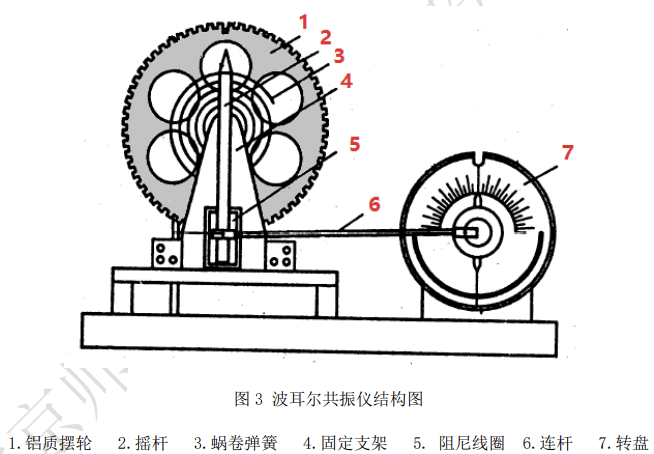
\includegraphics[width=0.7\textwidth]{apparatus.png}
    \caption{波耳共振仪结构图}
    \label{fig:apparatus}
\end{figure}

\subsection{实验步骤}
\subsubsection{衰减法测量振子的固有频率和品质因数}
\begin{enumerate}
    \item 不加驱动,阻尼线圈的电压从0-12V范围取值并固定。
    \item 手动让振子偏离平衡位置,然后释放,记录衰减振动曲线 $\theta(t)$。
    \item 用Capstone软件自带的“阻尼正弦” $\theta(t) = Ae^{-Bt} \sin(\omega t + \phi)$ 拟合实验数据。
    \item 根据拟合参数计算 $\omega_0$ 和 $Q$:
    \begin{equation}
    \omega_0 = \sqrt{\omega^2 + B^2}, \quad Q = \frac{\omega_0}{2B}
    \end{equation}
    \item 改变线圈电压,重复以上步骤。
\end{enumerate}

\subsubsection{测量电动机驱动信号频率($f$)与驱动圆频率 ($\omega$)之间的关系}
\begin{enumerate}
    \item 设定步进电动机的控制信号,输出1设为直流电压15V,输出2设为方波信号。
    \item 记录摇杆的角度变化曲线,用Capstone软件拟合实验数据,得到驱动频率 $\omega$。
    \item 多次改变电动机转速 $f$,测量相应驱动频率 $\omega$。
    \item 根据公式计算 $N = \frac{2\pi f}{\omega}$,并验证结果是否为常数。
\end{enumerate}

\subsubsection{稳态振动测量}
\begin{enumerate}
    \item 固定阻尼线圈电压,测量幅-频特性和相频特性曲线。
    \item 选择适当测量点,记录振动达到稳定后的数据。
    \item 改变阻尼线圈电压,重复测量,比较不同 $Q$ 值的频率特性曲线。
\end{enumerate}

\section{数据处理}
\begin{enumerate}
    \item 利用曲线拟合方法,从衰减振动曲线中提取参数,计算固有频率 $\omega_0$ 和品质因数 $Q$。
    \item 通过测量不同驱动频率下的稳态振幅,绘制幅频特性曲线和相频特性曲线,分析共振现象。
\end{enumerate}

\section{注意事项}
\begin{enumerate}
    \item 测量前确保传感器连接正常。
    \item 步进电动机通电前确认驱动电压的极性正确。
    \item 做受迫振动实验时必须加合适的阻尼,保证共振时摆轮的振幅不超过180度。
    \item 每次改变频率后,必须等足够长时间,达到稳态后再测量。
    \item 注意识别实验装置中存在的非线性因素。
\end{enumerate}




\bibliographystyle{plain}
\bibliography{./template}  %bib文件名

\end{document}
